%!TEX root = /Users/louis/Documents/PhD/Deliverables/Thesis/thesis.tex

\chapter{Background: Model-Driven Engineering}
\label{Background}
This chapter presents the thesis background, introduces concepts relating to Model-Driven Engineering (MDE), and surveys the MDE literature. Software evolution research is reviewed in Chapter~\ref{LiteratureReview}. MDE is a principled approach to software engineering in which models are produced and consumed throughout the engineering process. Section~\ref{sec:mde_terms} introduces the terminology and fundamental principles used in MDE. Section~\ref{sec:mde_methods} reviews guidance and three methods for performing MDE. Section~\ref{sec:mde_tools} describes contemporary MDE environments. Two areas of research relating to MDE, domain-specific languages and language-oriented programming, are discussed in Section~\ref{sec:mde_related}. Finally, the benefits of and current challenges for MDE are described in Section~\ref{sec:mde_benefits_and_challenges}.

%!TEX root = /Users/louis/Documents/PhD/Deliverables/Thesis/thesis.tex

\section{MDE Terminology and Principles}
\label{sec:mde_terms}
Software engineers using MDE construct and manipulate artefacts familiar from traditional approaches to software engineering (such as code and documentation) and, in addition, work with different types of artefact, such as \emph{models}, \emph{metamodels} and \emph{model transformations}. Furthermore, model-driven engineering involves new development activities, such as \emph{model management}. This section describes the artefacts and activities typically involved in a model-driven engineering process.

\subsection{Models} % TODO: review Jackson's and Kurtev's definitions of model
When used here, the term \emph{model} has the same meaning as given in \cite{kolovos06eol}: a model is a description of a phenomenon of interest, and may have either a textual or graphical representation. A model provides an abstraction over a real-world object, which enables engineers of differing disciplines to reason about that object.

Abstraction is the primary reason for and the primary goal of modelling. \cite{evans04domain} proposes the use of models throughout the development process to capture and communicate domain knowledge and to shape the structure of the resulting software. Evans emphasises the importance of modelling and a process, which he terms \emph{refactoring to deeper insight}, that seeks incremental improvements to models.

\begin{quote}
Distillation is the process of separating the components of a mixture to extract the essence in a form that makes it more valuable and useful. A model is a distillation of knowledge. With every refactoring to deeper insight, we abstract some crucial aspect of domain knowledge and priorities. \cite[pg397]{evans04domain}
\end{quote}

\cite[ch14]{martin06agile} notes that, in some engineering disciplines, models are used to reduce risk. Structural engineers build models of bridges. Aerospace engineers build models of aircraft. In these disciplines, a model is used to determine the efficacy of the real thing and, moreover, is cheaper to build and test than the real thing, often by a huge factor. The produce of many engineering disciplines is physical and the manufacturing process costly. Often, software models are not cheaper by a huge factor to build and test than the software they represent. Consequently, \cite[ch14]{martin06agile} prescribes software modelling for communicating and reasoning about a design, and not as a long-term replacement for real, working software.

All software has a \emph{domain}, the activities or business of its users. The domain of a library's lending system includes books, people and loans. \cite{evans04domain} prescribes principles and practices for building software in a way that emphasises the underlying domain, while tackling its complexity. In \cite{evans04domain}, domain models are key -- they are used to shape the solution's design, to define a common vocabulary for communication between team members, and to distinguish interesting and uninteresting elements of the domain. According to \cite{evans04domain}, domain models are key to software development. 

% Leading towards this argument:  Model-driven engineering provides principles and practices for defining and using modelling languages. A common metamodelling language is key. Is generative programming?

% How is the situation Martin describes (and other adovcates of "agile" principles) different to the software produced by model-driven engineering? Perhaps for enterprise systems it is much cheaper to build / test a model?? Or perhaps Martin is right, but MDD has different advantages to modelling (e.g. a common metamodelling language).

\subsection{Metamodelling}
In model-driven engineering, models are structured (conform to a well-defined set of syntactic and semantic constraints) rather than unstructured \cite{kolovos09thesis}. A \emph{modelling language} is the set of syntactic and semantic constraints used to define the structure of group of related models. In model-driven engineering, a modelling language is often specified as a model and, hence the term \emph{metamodel} is often used in place of \emph{modelling language}.

Metamodels facilitate model interchange and, hence, interoperability between modelling tools.  For this reason, Evans recommends that software engineers ``use a well-documented shared language that can express the necessary domain information as a common medium of communication.'' \cite[pg377]{evans04domain}. To support this recommendation, Evans discusses Chemical Markup Language (CML), a standardised language, which has facilitated the interoperability of tools (such as JUMBO Browser, which creates graphical views of chemical structures) developed by various institutions.

A metamodel typically comprises three categories of constraint:

\begin{itemize}
	\item \textbf{The concrete syntax} provides a notation for constructing models that conform to the language. For example, a model may be represented as a collection of boxes connected by lines. A standardised concrete syntax enables communication. Concrete syntax may be optimised for consumption by machines (e.g. XML Metadata Interchange (XMI) \cite{xmi}) or by humans (e.g. the concrete syntax of the Unified Modelling Language (UML) \cite{uml212}).
	\item \textbf{The abstract syntax} defines the concepts described by the language, such as classes, packages, datatypes. The representation for these concepts is independent of the concrete syntax. For example, compilers may elect to use an abstract syntax tree to encode the abstract syntax of a program (whereas the concrete syntax for the same language may be textual or diagrammatic).
	\item \textbf{The semantics} identifies the meaning of the modelling concepts in the particular domain of language. For example, consider a modelling language defined to describe genealogy, and another to describe flora. Although both languages may define a tree construct, the semantics of a tree in one is likely to be different from the semantics of a tree in the other. The semantics of a modelling language may be specified rigorously, by defining a reference semantics in a formal language such as Z \cite{z}, or in a semi-formal manner by employing natural language.
\end{itemize}

Concrete syntax, abstract syntax and semantics are used together to specify modelling languages. There are many other ways of defining languages, but this approach (first formalised in \cite{alvarez01mml}) is common in model-driven engineering: a metamodel is often used to define abstract syntax, a grammar or text-to-model transformation to specify concrete syntax, and code generators, annotated grammars or behavioural models to effect semantics.

\subsubsection{MOF}
Software engineers using model-driven engineering can use existing and define new metamodels. To facilitate interoperability between model-driven engineering tools, the OMG has standardised a language for specifying metamodels, the meta-object facility (MOF). Metamodels specified in MOF can be interchanged between model-driven engineering environments. Furthermore, modelling language tools are interoperable because MOF also standardises the way in which metamodels and their models are persisted to and from disk. For model and metamodel persistence MOF prescribes XML Metadata Interchange (XMI), a dialect of XML optimised and standardised by the OMG for loading, storing and exchanging models.

Because MOF is a modelling language for describing modelling languages, it is sometimes termed a metamodelling language. A simplified fragment of the UML defined in MOF, is shown in Figure \ref{fig:mof}. The concrete syntax of MOF borrows is similar to the concrete syntax of UML class diagrams:

\begin{itemize}
 \item Modelling constructs are drawn as boxes. The name of each modelling construct is emboldened. The name of abstract (uninstantiable) constructs are italicised.
 \item Attributes are contained within the box of their modelling construct. Each attribute has a name, a type (prefixed with a colon) and may define a default value (prefixed with an equals sign).
 \item Generalisation is represented using a line with an open arrow-head.
 \item References are specified using a line. An arrow illustrates the direction in which the reference may be traversed (no arrow indicates bi-directionality). Labels are used to name and define the multiplicity of references.
 \item Containment references are specified by including a solid diamond on the containing end.
\end{itemize}

\begin{figure}[htbp]
  \begin{center}
    \leavevmode
    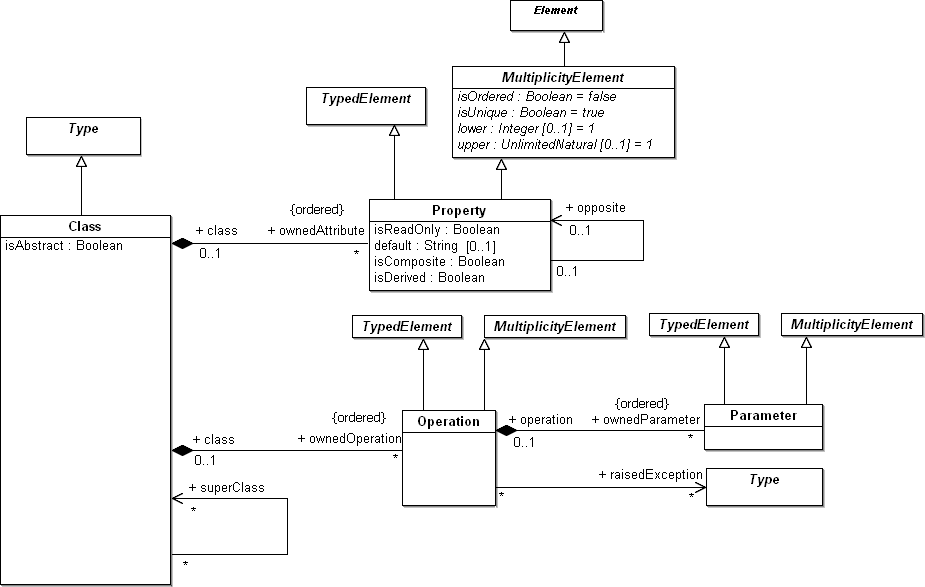
\includegraphics[scale=0.33]{mof.png}
  \end{center}
  \caption{A fragment of the UML metamodel defined in MOF, from \cite{uml212}.}
  \label{fig:mof}
\end{figure}

In the past, the means for describing modelling constructs has been inconsistent between modelling languages. For example, both entity-relationship (ER) diagrams and UML class diagrams can be used to specify models of structured data but, as \cite[pg97]{frankel02mda} notes, similar constructs from ER diagrams and UML class diagrams have different concrete syntax. MOF seeks to standardise the way in which modelling languages are defined.


\subsection{Model-Driven Engineering}
\label{sec:mde}
Model-driven engineering (MDE) is a principled approach to software engineering in which models are produced throughout the engineering process. Models are manipulated throughout development to produce software. This thesis uses the term \emph{model management}, defined in \cite{kolovos09thesis}, to refer to development activities that manipulate models for the purpose of producing software. Typical model management activities are discussed in this section.

\subsubsection{Model Transformation}
\label{subsubsec:model_transformation}
Model transformation is a development activity in which software artefacts are derived from others, according to some well-defined specification. Model transformations are specified between modelling languages (model-to-model transformation), between modelling languages and textual artefacts (model-to-text-transformation) and between textual artefacts and modelling languages (text-to-model transformation).

\cite{czarnecki06survey} survey describes a feature model for distinguishing and categorising model transformation approaches. Several of the features described by Czarnecki and Helsen are relevant to the research presented in this thesis, and are now discussed. 

% TODO Styles: imperative / hybrid / declarative 

Transformations specified between the same source and target metamodel are termed \emph{endogenous}, while transformation specified between different source and target metamodels are term \emph{exogenous}. Endogenous transformations can typically be specified with a more compact syntax than exogenous transformations, because there is no need to specify mappings between source and target types.

A \emph{new-target} transformation creates target models afresh on each invocation. An \emph{existing-target} transformation is executed on existing target models. Existing target transformations are used for partial (incremental) transformation and for preserving parts of the target that are not derived from the source.

Endogenous, existing-target transformations are used to perform small or incremental updates to models, such as refactorings, which will be discussed in Chapter~\ref{LiteratureReview}.


\paragraph{Model-to-Model (M2M) Transformation} M2M transformation has been characterised as the heart-and-soul of MDE \cite{sendall03heart}. Large and complex systems can be represented using several interdependent models. By automating the derivation of models from others, model transformation has the potential to reduce the cost of engineering large and complex systems.

\cite{kolovos08etl} notes that the current consensus is that hybrid languages, such as QVT \cite{qvt} and ATL \cite{jouault05transforming} are more suitable for specifying model transformation than pure imperative or declarative languages. 

\paragraph{Model-to-Text (M2T) Transformation} M2T transformation is an important model management task with a number of applications, including model serialisation (enabling model interchange); code and documentation generation; and model visualisation and exploration.  In 2005, the OMG \cite{omg} recognised the lack of a standardised in M2T transformation with its M2T Language Request for Proposals \footnote{\url{http://www.omg.org/docs/ad/04-04-07.pdf}}. In response, various M2T languages have been developed, including JET\footnote{\url{http://www.eclipse.org/modeling/m2t/?project=jet#jet}}, XPand\footnote{\url{http://www.eclipse.org/modeling/m2t/?project=xpand}} 
and MOFScript \cite{oldevik05toward}.

Because M2T transformation is used to produce unstructured artefacts, M2T transformation has different requirements to M2M transformation. For instance, code generators often provide mechanisms for specifying sections of code to be completed manually and for preserving those hand-written sections. Traceability between structured and unstructured artefacts is also a key requirement for model-to-text (and text-to-model) transformation, and is discussed further in Chapter~\ref{LiteratureReview}.

\paragraph{Text-to-Model (T2M) Transformation} T2M transformation is most often implemented as a parser that produces a model. Parser generators such as ANTLR \cite{parr07antlr} can be used to produce a structured artefact (such as an abstract syntax tree) from text. T2M tools are built atop parser generators and post-process the structured artefacts such that they conform to the target metamodel. Xtext \footnote{\url{http://www.eclipse.org/Xtext/}} and EMFtext \cite{heidenreich09derivation} are contemporary examples of T2M tools that, given a grammar and a target metamodel, will automatically generate a parser that transforms text to a model.

\subsubsection{Model Validation}
Model validation provides a mechanism for managing the integrity of the software developed using MDE. A model that omits information is said to be \emph{incomplete}, while related models that suggest differences in the underlying phenomena are said to be \emph{contradicting}. Incompleteness and contradiction are two examples of \emph{inconsistency}. In MDE, inconsistency is detrimental, because, when artefacts are automatically derived from each other, the inconsistency of one artefact might be propagated to others. Model validation is used to detect, report and reconcile inconsistency throughout a MDE process.

\cite{kolovos09thesis} observes that inconsistency detection is inherently pattern-based and, hence, higher-order languages are more suitable for model validation than 3G languages (such as Java). The Object Constraint Language (OCL) \cite{ocl2}, an OMG standard, can be used to specify consistency constraints on UML and MOF models. Unlike OCL, the xlinkit toolkit \cite{nentwich2003flexible} can be used for specifying inter-model consistency constraints. 

\subsubsection{Further model management activities}
In addition to model transformation and validation, further examples of model management activities include model comparison (e.g. \cite{kolovos06ecl}), in which a \emph{trace} of similar and different elements is produced from two or more models, and model merging or weaving (e.g. \cite{kolovos07eml}), in which a two or more models are combined to produce a unified model.

Further activities, such as model versioning and tracing, might be regarded as model management but, in the context of this thesis, are considered as evolutionary activities and as such are discussed in Chapter~\ref{LiteratureReview}.

\subsection{Summary}
This section has introduced the terminology and principles necessary for discussing MDE in this thesis. Models provide abstraction, capturing necessary and disregarding irrelevant details. Metamodels provide a structured mechanism for describing the syntactic and semantic rules to which a model most conform. Metamodels facilitate interoperability between modelling tools and MOF, the OMG standard metamodelling language, enables the development of tools that can be used with a range of metamodels, such as model management tools. Throughout model-driven engineering, models are manipulated to produce other development artefacts using model management activities such as model transformation and validation. Using the terms and principles described in this section, the ways in which model-driven engineering is performed in practice are now discussed.
%!TEX root = /Users/louis/Documents/PhD/Deliverables/Thesis/thesis.tex

\section{MDE Methods}
\label{sec:mde_methods}
For performing model-driven engineering, new practices and processes have been proposed. Proponents of MDE have produced guidance and methods for model-driven engineering. This section discusses the guidance for MDE set out in the Model-Driven Architecture \cite{mda} and the methods described by \cite{stahl06mdsd,kelly08dsm,greenfield04software}. 

\subsection{Model-Driven Architecture (MDA)}
Model-Driven Architecture (MDA) is a software engineering framework defined by the OMG. MDA provides a set of guidelines for model-driven engineering. MDA prescribes the use of a Platform Independent Model (PIM) and one or more Platform Specific Models (PSMs).

A PIM provides an abstract, implementation-agnostic view of the solution. Successive PSMs provide increasingly more implementation detail. Inter-model mappings are used to forward- and reverse-engineer these models, as depicted in
Figure \ref{fig:mda}.

\begin{figure}[htbp]
  \begin{center}
    \leavevmode
    \includegraphics[scale=0.5]{MDA.png}
  \end{center}
  \caption{Interactions between a PIM and several PSMs.}
  \label{fig:mda}
\end{figure}

The crucial difference between MDA and related approaches, such as round-trip engineering (in which models and code are co-evolved to develop a system), is that traditional round-trip engineering uses some manual transformations, whereas MDA prescribes automated transformations between PIM and PSMs.

McNeile \cite{mcneile03mda} identifies two ways in which engineers are utilising MDA. Both interpretations begin with a PIM and vary in the way they are used to produce executable code:

\begin{itemize}
 \item \textbf{Translationist}: The PIM is used to generate code directly using a sophisticated code generator. Any intermediate PSMs are internal to the code generator. No generated artefacts are edited manually.
 \item \textbf{Elaborationist}: Any generated artefacts (such as PSMs, code and documentation) can be augmented with further details of the application. To ensure that all models and code are synchronised, tools must allow bi-directional transformations.
\end{itemize}

Translationists must encode behaviour in their PIMs \cite{mellor02executable}, whereas elaborationists have a choice, frequently electing to specify behaviour in PSMs or in code \cite{kleppe03mda}.

The MDA prescribes a set of standards for MDE. The MDA allocates standards to one of four tiers, representing different levels of model abstraction. Members of each tier are instances of the members of parent tiers. These tiers can be seen in Figure \ref{fig:mda-pyramid}, and a short discussion based on \cite[Section 8.2]{kleppe03mda} follows.

\begin{figure}[htbp]
  \begin{center}
    \leavevmode
    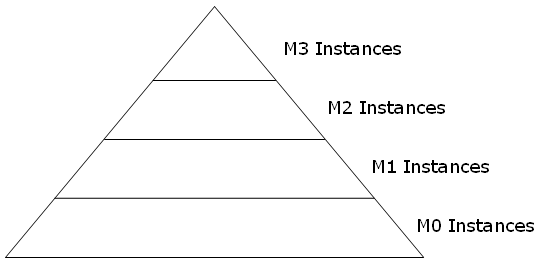
\includegraphics[scale=0.5]{mda-pyramid.png}
  \end{center}
  \caption{The tiers of standards used as part of MDA.}
  \label{fig:mda-pyramid}
\end{figure}

The base of the pyramid, tier M0, describes the real-world. When modelling a business, this tier is used to describe items of the business itself, such as a real customer or an invoice. When modelling software, M0 instances describe the software representation of such items. M1 contains a model of the concepts in M0, for example a customer may be represented as a class with attributes. The M2 tier describes the model of the modelling language used to describe elements of M1. For example, if UML \cite{uml212} were used to describe concepts as classes in the M1 tier, M2 would contain the UML metamodel. Finally, M3 is the meta-metamodel layer, which provides a description of the metamodel used in M2. M3 is necessary to permit reasoning about metamodels (such as the UML), and to enable tool standardisation. The OMG defines the Meta-Object Facility (MOF) \cite{mof} as the sole inhabitant of the M3 tier.


\subsection{Methods for MDE}
Several methods to MDE are prevalent today. In this section, three of the most established are discussed: Architecture-Centric Model-Driven Software Development \cite{stahl06mdsd}, Domain-Specific Modelling \cite{kelly08dsm} and Microsoft's Software Factories \cite{greenfield04software}. All three methods have been defined from a pragmatic standpoint (i.e. they have been used repeatedly to solve problems in industry). The methods vary in the extent to which they follow the guidelines set out by MDA.

\subsubsection{Architecture-Centric Model-Driven Software Development}
Model-Driven Software Development is the term given to MDE by in \cite{stahl06mdsd}. The style of MDE that Stahl et al. describe, \textit{architecture-centric model-driven software development} (AC-MDSD), focuses on generating the infrastructure of large-scale applications. For example, a typical J2EE application contains concepts (such as EJBs, descriptors, home and remote interfaces) that ``admittedly contain domain-related information such as method signatures, but which also exhibit a high degree of redundancy'' \cite{stahl06mdsd}. It is this redundancy that AC-MDSD seeks to remove by using code generators, requiring only the domain-related information to be specified.

AC-MDSD applies more of the MDA guidelines than the other methods discussed below. For instance, AC-MDSD supports the use of a general-purpose modelling language for specifying models. \cite{stahl06mdsd} utilise UML in many of their examples, which demonstrate how AC-MDSD may be used to enhance the productivity, efficiency and understandability of software development. In these examples, models are annotated using UML profiles to describe domain-specific concepts.


\subsubsection{Domain-Specific Modelling}
\cite{kelly08dsm} present a method for MDE termed Domain-Specific Modelling (DSM). DSM is based on the translationist interpretation of MDA; DSM seeks to translate models containing concepts from the problem domain to full code. In motivating the need for DSM, Kelly and Tolvanen state that large productivity gains were made when third-generation programming languages were used in place of assembler, and that no paradigm shift has since been able to replicate this degree of improvement. Tolvanen\footnote{Tutorial on Domain Specific Modelling for Full Code Generation at the Fourth European Conference on Model Driven Architecture (ECMDA), June 2008, Berlin, Germany.} notes that DSM focuses on increasing the productivity of software engineering by allowing developers to specify solutions by using models that describe the application domain.

To perform DSM, expert developers define:

\begin{itemize}
 \item \textbf{A domain-specific modelling language}: allowing domain experts to encode solutions to their problems.
 \item \textbf{A code generator}: that translates the domain-specific models to executable code in an existing programming language.
 \item \textbf{Framework code}: that encapsulates the common areas of all applications in this domain.
\end{itemize}

As the development of these three artefacts requires significant effort from expert developers, Tolvanen\footnotemark[\value{footnote}] states that DSM should only be applied if more than three problems specific to the same domain are to be solved.

Tools for defining domain-specific modelling languages, editors and code generators enable DSM \cite{kelly08dsm}. Reducing the effort required to specify these artefacts is key to the success of DSM. In this respect, DSM resembles a programming paradigm popular in the \textit{domain-specific language} (DSL) community, termed \textit{language-oriented programming} (LOP), which also requires tools to simplify the specification of new languages. DSLs and LOP are discussed further in Section \ref{sec:mde_related}.

Throughout \cite{kelly08dsm}, examples from industrial partners are used to illustrate that DSM can greatly improve developer productivity. Unlike MDA, DSM seems to be optimised for increasing productivity, and less concerned with portability or maintainability. Therefore, DSM is less suitable for engineering applications that frequently interoperate with -- and are underpinned by -- changing technologies.

\subsubsection{Microsoft Software Factories}
Greenfield \cite[pg159]{greenfield04software} states that industrialisation of the automobile industry has addressed problems with economies of scale (mass production) and scope (product variation). Software Factories, a software engineering method developed at Microsoft, seek to address problems with economies of scope in software engineering by borrowing concepts from product-line engineering. Greenfield \cite{greenfield04software} argues that, unlike many other engineering disciplines, software development requires considerably more development effort than production effort in that scaling software development to account for scope is significantly more complicated then mass production of the same software system.

The Software Factories method \cite{greenfield04software} prescribes a bottom-up approach to abstraction and re-use. Development begins by producing prototypical applications. The common elements of these applications are identified and abstracted into a product-line. When instantiating a product, models are used to specify product variance (e.g. by selecting particular product features). To generate these models, tools for use with Software Factories provide mechanisms for defining wizards and feature-based configuration selection dialogues. By contrast, DSM relies upon the use of concrete syntax for producing models that describe product variance. By providing explanations that assist in making decisions, the wizards used in Software Factories guide users towards best practices. Greenfield et al. state that ``moving from totally-open ended hand-coding to more constrained forms of specification [such as wizard-based feature selection] are the key to accelerating software development'' \cite[pg179]{greenfield04software}.

The Software Factories method better addresses problems of portability compared to DSM: the former provides \textit{viewpoints} into the product-line (essentially different views of development artefacts), which allow decoupling of concerns (e.g. between logical, conceptual and physical layers). Viewpoints provide a mechanism for abstracting over different layers of platform independence, adhering more closely than DSM to the guidelines provided in MDA. Unlike the guidelines provided in MDA, the Software Factories method does not insist that development artefacts be derived automatically where possible.

Finally, Microsoft prescribes the use of domain-specific languages (discussed in Section \ref{LitReview:DSLs}) for describing models in conjunction with Software Factories, rather than a general-purpose modelling language, as Microsoft believes that the latter often have imprecise semantics \cite{greenfield04software}.

\subsection{Summary}
This section has discussed the ways in which process and practices for MDE have been captured. Guidance for MDE has been set out in the MDA standard, which seeks to use MDE to produce adaptable software in a productive and maintainable manner. Three methods for performing model-driven engineering have been discussed.
 
The methods discussed share some characteristics. They all require a set of exemplar applications, which are examined by MDE experts. Analysis of the exemplar applications identifies the way in which software development may be decomposed. A modelling language for the problem domain is constructed, and instances are used to generate future applications. Code common to all applications in the problem domain is encapsulated into a framework.

Each method has a different focus. AC-MDSD seeks to reduce the amount of boilerplate code being generated, particularly in enterprise applications. Software Factories concentrate on providing different viewpoints into the system, allowing different domain experts to collaborate when specifying a system. DSM aims to decrease the time taken to develop software solutions to instances of the problem domain.

Perhaps unsurprisingly, the proponents of each method for MDE recommend one or more tools, each optimised for that method (such as MetaCase for DSM). Alternative tools are available from open-source modelling communities, including the Eclipse Modelling Project, which provides -- among other tools for MDE -- arguably the most widely used MDE modelling framework today. Some of the tools used for MDE are reviewed in the sequel.
%!TEX root = /Users/louis/Documents/PhD/Deliverables/Thesis/thesis.tex

\section{Tools for MDE}
\label{sec:mde_tools}
Mature and powerful tools and languages for many common MDE activities are available today. This section discusses two MDE tools that are well-suited for MDE research and that are used in the remainder of the thesis.

Section~\ref{subsec:emf} provides an overview of the Eclipse Modelling Framework (EMF) \cite{steinberg09emf}, which implements MOF and underpins many contemporary MDE tools and languages, facilitating their interoperability. Section~\ref{subsec:epsilon} discusses Epsilon \cite{kolovos09thesis}, an extensible platform for the specification of model management languages. The highly extensible nature of Epsilon (which is described below) makes it an ideal host for the rapid prototyping of languages and exploring research hypotheses.  

The purpose of this section is to review EMF and Epsilon, and not to provide a thorough review of all MDE tools. There are many other MDE tools and environments that this section does not discuss, such as ATL and VIATRA for M2M transformation (Section~\ref{subsubsec:model_transformation}), oAW\footnote{\url{http://www.eclipse.org/workinggroups/oaw/}} for model transformation and validation, and the AMMA platform\footnote{\url{http://wiki.eclipse.org/AMMA}} for large-scale modelling, model weaving and software modernisation.

\subsection{Eclipse Modelling Framework}
\label{subsec:emf}
The Eclipse Foundation\footnote{\url{http://www.eclipse.org}} is an open-source community seeking to build an extensible development platform. The Eclipse Modelling Framework (EMF) project \cite{steinberg09emf} provides support for MDE within Eclipse. EMF provides code generation facilities, and a meta-modelling language, Ecore, that implements the MOF 2.0 standard \cite{mof}. EMF is arguably the most widely-used contemporary MDE modelling framework.

EMF is used to generate metamodel-specific editors for loading, storing and constructing models. EMF model editors comprise a navigation view for specifying the elements of the model, and a properties view for specifying the features of model elements. Figure~\ref{fig:emf_model_editor} shows an EMF model editor for a simple state machine language. The navigation (or tree) view is shown in the top pane, while the properties view is shown in the bottom pane.

\begin{figure}[htbp]
  \begin{center}
    \leavevmode
    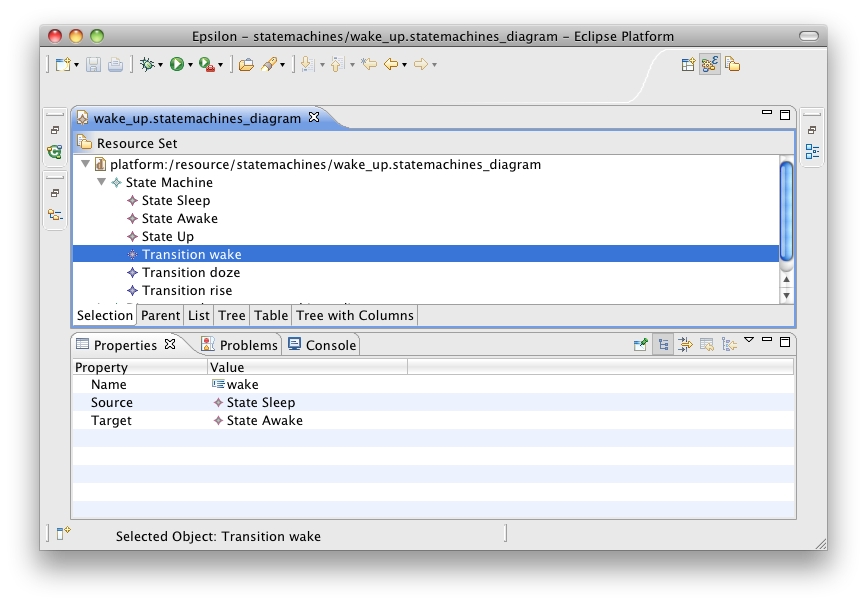
\includegraphics[width=10cm]{2.Background/images/emf_model_editor.png}
  \end{center}
  \caption{An EMF model editor for state machines.}
  \label{fig:emf_model_editor}
\end{figure}

Users of EMF can define their own metamodels in Ecore, the metamodelling language and MOF implementation of EMF. EMF provides two metamodel editors, tree-based and graphical. Figure~\ref{fig:emf_metamodel_editor_tree} shows the metamodel of a simple state machine language in the tree-based metamodel editor. Figure~\ref{fig:emf_metamodel_editor_diagrammatic} shows the same metamodel in the graphical metamodel editor. Like MOF, the graphical metamodel editor uses concrete syntax similar to that of UML class diagrams. Emfatic\footnote{\url{http://www.alphaworks.ibm.com/tech/emfatic}} provides a further, textual metamodel editor for EMF, and is shown in Figure~\ref{fig:emf_metamodel_editor_textual}. The editors shown in Figure~\ref{fig:emf_metamodel_editor_tree}, \ref{fig:emf_metamodel_editor_diagrammatic} and \ref{fig:emf_metamodel_editor_textual} are used to manipulate the same underlying metamodel, but using different syntaxes. A change to the metamodel in one editor can be propagated automatically to the other two.

\begin{figure}[htbp]
  \begin{center}
    \leavevmode
    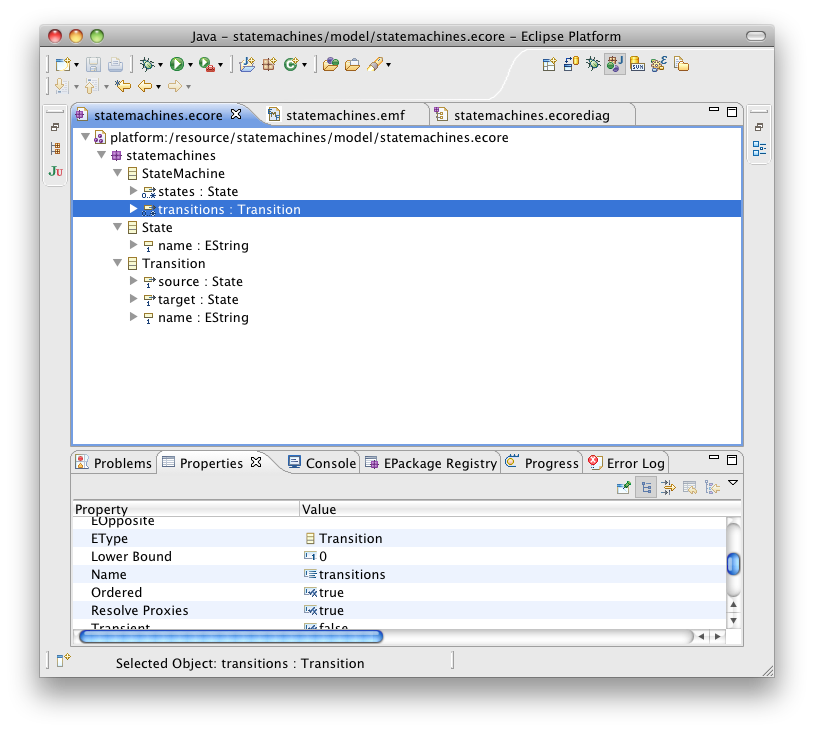
\includegraphics[width=10cm]{2.Background/images/emf_metamodel_tree.png}
  \end{center}
  \caption{EMF's tree-based metamodel editor.}
  \label{fig:emf_metamodel_editor_tree}
\end{figure}

\begin{figure}[htbp]
  \begin{center}
    \leavevmode
    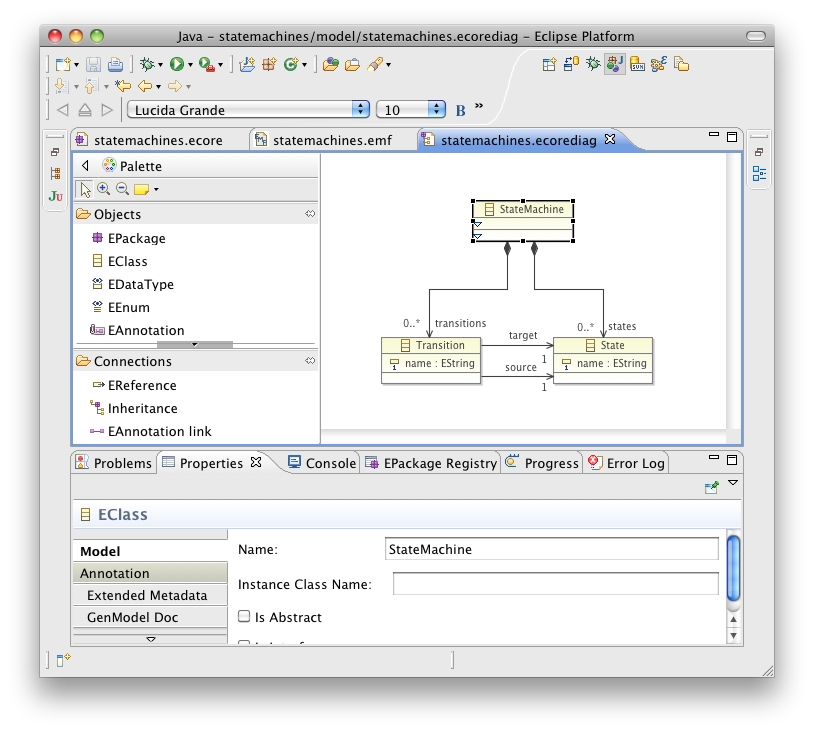
\includegraphics[width=10cm]{2.Background/images/emf_metamodel_diagrammatic.png}
  \end{center}
  \caption{EMF's graphical metamodel editor.}
  \label{fig:emf_metamodel_editor_diagrammatic}
\end{figure}

\begin{figure}[htbp]
  \begin{center}
    \leavevmode
    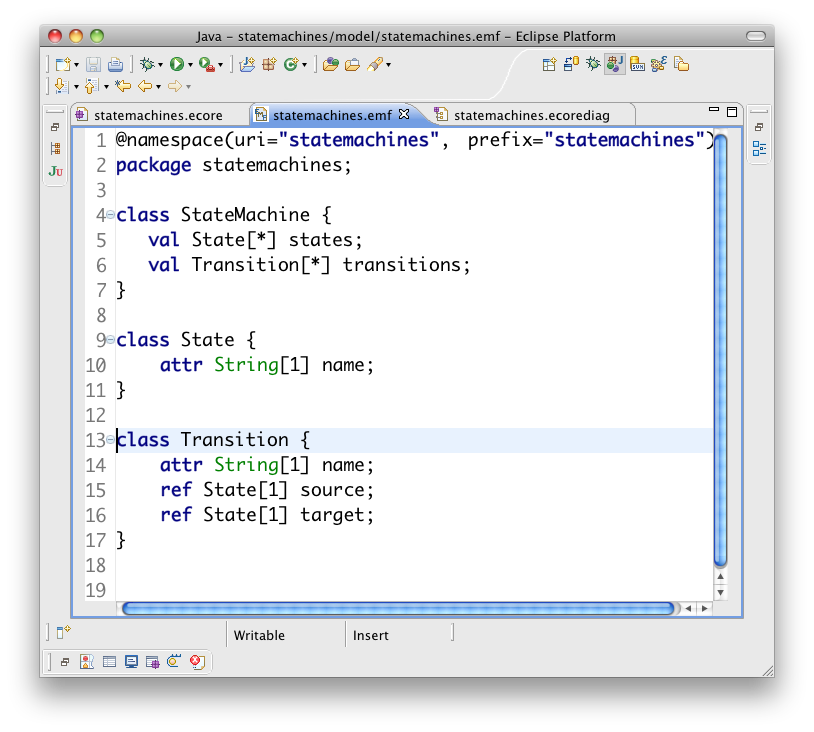
\includegraphics[width=10cm]{2.Background/images/emf_metamodel_textual.png}
  \end{center}
  \caption{The Emfatic textual metamodel editor for EMF.}
  \label{fig:emf_metamodel_editor_textual}
\end{figure}

From a metamodel, EMF can generate an editor for models that conform to that metamodel. For example, the simple state machine metamodel specified in Figures~\ref{fig:emf_metamodel_editor_tree}, \ref{fig:emf_metamodel_editor_diagrammatic} and \ref{fig:emf_metamodel_editor_textual} was used to generate the code for the model editor shown in Figure~\ref{fig:emf_model_editor}. The model editors generated by EMF incorporate mechanisms for loading and saving models. As prescribed by MOF, EMF typically generates code that stores models using XMI \cite{xmi}, a dialect of XML optimised for model interchange.

The Graphical Modeling Framework (GMF) \cite{gronback09emp} is used to create graphical model editors from metamodels defined with EMF. Figure~\ref{fig:gmf_model_editor} shows a model editor produced with GMF for the simple state machine language described above. GMF itself uses a model-driven approach: users specify several models, which are combined, transformed and then used to generate code for the resulting graphical editor. 

\begin{figure}[htbp]
  \begin{center}
    \leavevmode
    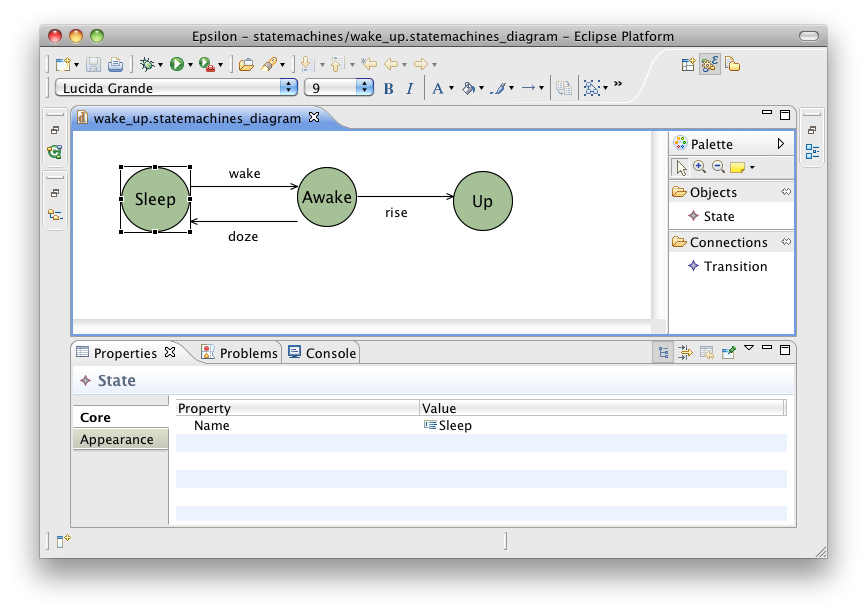
\includegraphics[width=10cm]{2.Background/images/gmf_model_editor.png}
  \end{center}
  \caption{GMF state machine model editor.}
  \label{fig:gmf_model_editor}
\end{figure}

Many MDE tools are interoperable with EMF, enriching its functionality. The remainder of this section discusses one tool that is interoperable with EMF, Epsilon.

\subsection{Epsilon}
\label{subsec:epsilon}
The Extensible Platform for Specification of Integrated Languages for mOdel maNagement (Epsilon) \cite{kolovos09thesis} is a suite of tools and domain-specific languages for MDE. Epsilon comprises several integrated model management languages -- built on \changed{``atop'' to ``on''} a common infrastructure -- for performing tasks such as model transformation, model validation and model merging \cite{kolovos09thesis}. Figure \ref{fig:epsilon} illustrates the various components of Epsilon.

Whilst many model management languages are bound to a particular subset of modelling technologies, limiting their applicability, Epsilon is metamodel-agnostic: models written in any modelling language can be manipulated by Epsilon's model management languages \cite{kolovos06eol}. Currently, Epsilon supports models implemented using EMF, MOF 1.4, XML, or Community Z Tools (CZT)\footnote{\url{http://czt.sourceforge.net/}}. Interoperability with further modelling technologies can be achieved by extension of the Epsilon Model Connectivity (EMC) layer. 

\begin{figure}[htbp]
  \begin{center}
    \leavevmode
    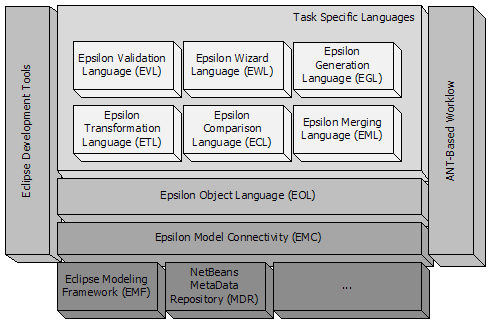
\includegraphics[scale=0.6]{2.Background/images/epsilon.png}
  \end{center}
  \caption[The architecture of Epsilon]{The architecture of Epsilon, taken from \cite{rose08egl}.}
  \label{fig:epsilon}
\end{figure}

The architecture of Epsilon promotes reuse when building task-specific model management languages and tools. Each Epsilon language can be reused wholesale in the production of new languages. Ideally, the developer of a new language only has to design language concepts and logic that do not already exist in Epsilon languages. As such, new task-specific languages can be implemented in a minimalistic fashion. This \cc claim has been demonstrated by the style of implementation used to construct the Epsilon Generation Language (EGL) \cite{rose08egl}.

The Epsilon Object Language (EOL) \cite{kolovos06eol} is the core of the platform and provides functionality similar to that of OCL \cite{ocl2}. However, EOL provides an extended feature set, which includes the ability to update models, access to multiple models, conditional and loop statements, statement sequencing, and provision of standard output and error streams.

As shown in Figure \ref{fig:epsilon}, every Epsilon language re-uses EOL, so improvements to EOL enhance the entire platform. EOL also allows developers to delegate computationally intensive tasks to extension points, where the task can be authored in Java.

Epsilon is a member of the Eclipse GMT\footnote{\url{http://www.eclipse.org/gmt}} project, a research incubator for the top-level modelling technology project. Epsilon provides a lightweight means for defining new experimental languages for MDE. For these reasons, Epsilon is uniquely positioned as an ideal host for the rapid prototyping of languages for model management, and hence has been used extensively for the work described in Chapter~\ref{Implementation}. 

\subsection{Summary}
This section has introduced the MDE tools used throughout the remainder of the thesis. The Eclipse Modeling Framework (EMF) provides an implementation of MOF, Ecore, for defining metamodels. From metamodels defined in Ecore, EMF can generate code for metamodel-specific editors and for persisting models to disk. EMF is arguably the most widely used contemporary MDE modelling framework and its functionality is enhanced by numerous tools, such as the Graphical Modeling Framework (GMF) and Epsilon. GMF allows metamodel developers to specify a graphical concrete syntax for metamodels, and can be used to generate graphical model editors. Epsilon is an extensible platform for defining and executing model management languages, provides a high degree of re-use for defining new model management languages and can be used with a range of modelling frameworks, including EMF.
%!TEX root = /Users/louis/Documents/PhD/Deliverables/Thesis/thesis.tex

\section{Research Relating to MDE}
\label{sec:mde_related}
MDE is closely related to several other fields of software engineering. This section discusses two of those fields, Domain-Specific Languages (DSLs) and Language-Oriented Programming (LOP). A further related area, Grammarware, is discussed in the context of software evolution in Section~\ref{subsec:grammar_evolution}. DSLs and LOP are closely related to the research central to this thesis. Other areas relating to MDE but less relevant to this thesis, such as formal methods, are not considered here.

\subsection{Domain-Specific Languages}
\label{subsec:dsls}
For a set of closely-related problems, a specific, tailored approach is likely to provide better results than instantiating a generic approach for each problem \cite{deursen00dslbib}. The set of problems for which the specific approach outperforms the generic approach is termed the \emph{domain}. A \emph{domain-specific programming language} (often called a \emph{domain-specific language} or \emph{DSL}) enables the encoding of solutions for a particular domain.

Like modelling languages, DSLs describe abstract syntax. Furthermore, a common language can be used to define DSLs (e.g. EBNF \cite{ebnf}), like the use of MOF for defining modelling languages. In addition to abstract syntax, DSLs typically define a textual concrete syntax but, like modelling languages, can utilise a graphical concrete syntax.

Cobol, Fortran and Lisp first existed as DSLs for solving problems in the domains of business processing, numeric computation and symbolic processing respectively, and evolved to become general-purpose programming languages \cite{deursen00dslbib}. SQL, on the other hand, is an example of a DSL that, despite undergoing much change, has not grown into a general-purpose language. Unlike a general-purpose language, a single DSL cannot be used to program an entire application. DSLs are often small languages at inception, but can grow to become complicated (such as SQL). Within their domain, DSLs should be easy to read, understand and edit \cite{fowler10dsls}.

There are two ways in which DSLs are typically implemented. An \emph{internal} DSL uses constructs from a general-purpose language (the \emph{host}) to describe the domain \cite{fowler10dsls}. Examples of internal DSLs include the libraries of abstract data types that are part of many programming languages (e.g. STL for C++, the Collections API for Java). Some languages are better than others for hosting internal DSLs. For example, \cite{fowler10dsls} proposes Ruby as a suitable host for DSLs due to its ``unintrusive syntax and flexible runtime evaluation.'' \cite{graham93lisp} describes a technique for implementing internal DSLs in Lisp, in which macros are used to translate domain-specific concepts to Lisp abstractions.

When the gap between domain and programming concepts is large, constructing an internal DSL can require a lot of programming effort. For this reason, \cite{parr07antlr} advocates the implementation of DSLs by \emph{translating} DSL programs into code written in a general-purpose language. \cite{fowler10dsls} uses the term \emph{external} for this style of DSL implementation. Programs written in simple DSLs are often easy to translate to programs in an existing general-purpose language \cite{parr07antlr}. Approaches to translation include preprocessing; building or generating an interpreter or compiler; or extending an existing compiler or interpreter \cite{fowler10dsls}.

The construction of an external DSL can be achieved using many of the principles, practices and tools used in MDE. Parsers can be generated using text-to-model transformation; syntactic constraints can be specified with model validation; and translation can be specified using model-to-model and model-to-text transformation. MDE tools are used to implement two external DSLs in Chapter~\ref{Implementation}.

Internal and external DSLs have been successfully used as part of application development in many domains, as described in \cite{deursen00dslbib}. They have been used in conjunction with general-purpose languages to build systems rapidly and to improve productivity in the development process (such as automation of system deployment and configuration). More recently, some developers are building complete applications by combining DSLs, in a style of development called Language-Oriented Programming. 

\subsection{Language-Oriented Programming (LOP)}
DSLs are central to LOP, a style of software development. \cite{ward94lop} describes the key tenets of a LOP process. Firstly, a very high-level language to encode problem domains is developed. Simultaneously, a compiler is developed to translate programs written in the high-level language to an existing programming language. Ward describes how this approach to programming can enhance the productivity of development and the understandability of a system. Additionally, Ward mentions the way in which multiple very high-level languages could be layered to separate domains.

The high-level languages that Ward discusses are domain-specific. \cite{fowler10dsls} notes that combining DSLs to solve a problem is not a new technique. Traditionally, UNIX has encouraged developers to combine programs written in small (domain-specific) languages (such as awk, make, sed, lex and yac) to solve problems. Lisp, Smalltalk and Ruby programmers often construct domain-specific languages when developing programs \cite{graham93lisp}.

To fully realise the benefits of LOP, the development effort required to construct DSLs must be minimised. Two approaches for constructing DSLs seem to be prevalent for LOP. The first advocates using a highly dynamic, reflexive and extensible programming language to specify DSLs. \cite{clark08superlanguages} terms this category of language a \textit{superlanguage}. The superlanguage permits new DSLs to re-use constructs from existing DSLs, which simplifies development.

A \textit{language workbench} \cite[ch. 9]{fowler10dsls} is an alternative means for simplifying DSL development. Language workbenches provide tools, wizards and DSLs for defining abstract and concrete syntax, for constructing editors and for specifying code generators.

For defining DSLs, the main difference between using a language workbench or a superlanguage is the way in which semantics of language concepts are encoded. In a language workbench, a typical approach is to write a generator for each DSL \cite{fowler10dsls}, whereas a superlanguage often requires that semantics be encoded in the definition of language constructs \cite{clark08superlanguages}.

Like MDE, LOP requires mature and powerful tools and languages to be applicable in the large, and to complex systems. Unlike MDE, LOP tools typically combine concrete and abstract syntax. The emphasis for LOP is in defining a single, textual concrete syntax for a language. MDE tools might provide more than one concrete syntax for a single modelling language. For example, two distinct concrete syntaxes are used for the tree-based and graphical editors of the simple state-machine language shown in Figures~\ref{fig:emf_model_editor} and~\ref{fig:gmf_model_editor}.

Some of the key concerns for MDE are also important to the success of LOP. For example, tools for performing LOP and MDE need to be as usable as those available for traditional development, which often include support for code-completion, automated refactoring and debugging. Presently, these features are often lacking in tools that support LOP or MDE.

In summary, LOP addresses many of the same issues with traditional development as MDE, but requires a different style of tool. LOP focuses more on the integration of distinct DSLs, and providing editors and code generators for them. Compared to LOP, MDE typically provides more separation between concrete and abstract syntax, and concentrates more on model management.

\subsection{Summary}
This section has described two areas of research related to MDE, domain-specific languages (DSLs) and language-oriented programming (LOP). DSLs facilitate the encoding of solutions for a particular problem domain. For solving problems in their domain, DSLs can be easier to read, use and edit than general-purpose programming languages \cite{deursen00dslbib,fowler10dsls}. During MDE, one or more DSLs may be used to model the domain, and the tools and techniques for implementing DSLs can be used for MDE.

LOP is an approach to software development that seeks to specify complete systems using a combination of DSLs. Contemporary LOP seeks to minimise the effort required to specify and use DSLs. Like MDE, LOP requires mature and powerful tools, but, unlike MDE, LOP does not separate concrete and abstract syntax, and does not focus on model management, which is a key development activity in MDE.

%!TEX root = /Users/louis/Documents/PhD/Deliverables/Thesis/thesis.tex

\section{Benefits of and Current Challenges for MDE}
\label{sec:mde_benefits_and_challenges}

\subsection{Benefits}
Modelling allows software engineers to capture concepts of interest and simultaneously disregard superfluous detail. Proponents of MDE use models to increase the extent to which software systems exhibit characteristics they find desirable. For example, the guidelines set out for MDE in MDA \cite{mda} highlight principles and patterns for modelling to increase the adaptability of software systems by, for example, separating platform-specific and platform-independent detail. When the target platform changes (for example a new technological architecture is required), only part of the system needs to be changed.
%(But, in practice, is this separation always desirable / achievable?)

MDE facilitates automation of the error-prone or tedious elements of software engineering. For example, code generation can be used to automatically produce 
``boilerplate'' code % explain boilerplate code

For software systems that must incorporate large-scale complexity, such as those that support large businesses, managing stochastic interaction in-the-large is a key concern. With MDE it is possible to sacrifice total reliability or validity of a system to achieve a working solution. Sacrificing reliability or validity is not always possible when other engineering approaches are used to construct software (such as formal methods). 

MOF, the standard metamodelling language for MDE, facilitates interoperability between tools via model interchange. In Ecore, EMF provides a reference implementation of MOF atop which many MDE tools are built. There are, however, many further ways in which MDE tools might usefully interoperate, which are discussed, along with other challenges for MDE, in the sequel.

\subsection{Challenges}

Start-up hurdle
Tools more than theory (modelling is relatively accessible)
Legacy issue: some capabilities not yet well integrated with MDE tools (e.g. refactoring, version control)
Learning curve can be very steep (huge effort for first, trivial result). Particularly apparent in GMF.
Businesses might put one person (and usually not their best person) on exploring new technology.
Bad first experience causes low adoption rates.
Potential solutions: more examples (what's the MDE "hello world"?), automation for complicated tasks
Danger of MDE becoming a purely academic endeavour?
Academic advances should be linked to commercial realities
Formal methods have had some success here
Open-source helps to encourage commercial activity (but there are often concerns about support / bug fixing)
Code generation vs runtime models
Is code generation less important when one language is used? Some libraries use one language to abstract over others, for example Google Web Toolkit (all code written in Java, and source is compiled to HTML and Javascript).
Here much of the model is in the code, and we're back to the problem of "does my model match my code?"
Code generation often requires an elaborate software architecture that facilitates the mixing of generated and hand-written code.
Perception
In some situations, using MDE produces more artefacts (which have to be maintained)
Confusion between tools: What is Eclipse? What is EMF? Where are the boundaries? How decoupled are the tools?
Do we need something between a heavyweight method and freeform hacking? For example, process patterns that recommend useful combinations of MDE tools.
Interoperability of MDE tools
Good interoperability of terms of model interchange, but tighter integration might be necessary
Open-source helps: use a suitable tool, rather than an unsuitable tool to validate the cost of the license

\subsubsection{Scalability}
In traditional approaches to software engineering, a model is considered of comparable value to any other documentation artefact, such as a word processor document or a spreadsheet. As a result, the convenience of maintaining self-contained model files which can be easily shared outweighs other desirable attributes. This perception has led to the current situation where single-file models of the order of tens (if not hundreds) of megabytes, containing hundreds of thousands of model elements, are the norm for real-world software projects \cite{kolovos08scalability}.

In model-driven engineering, a model is a development artefact and, while sharing models with others is still a concern, other attributes are desirable. Modularity, for example, is important for supporting incremental transformation and collaborative development \cite{kolovos08scalability}.

MDE languages and tools must be usable with with large and complex models...


\subsubsection{Resistance to change}

\section{Chapter Summary}
This chapter has discussed Model-Driven Engineering (MDE), a state-of-the-art and principled approach to software engineering. The terminology, development activities and tools used in a typical MDE process were introduced. Two areas relating to MDE, language-oriented programming and domain-specific languages, were discussed, and three methods for performing MDE were reviewed.

Traditional approaches to software engineering do not treat modelling artefacts -- such as model, metamodels and model management operations -- as first-class citizens, and they are typically represented in an unstructured manner, if at all. MDE involves creating, manipulating and managing changes to modelling artefacts and therefore modelling artefacts are represented in a structured manner. This chapter has demonstrated that contemporary MDE tools, such as EMF and Epsilon, provide structures and processes for creating and manipulating modelling artefacts, but not for managing evolutionary change. Chapters~\ref{LiteratureReview} and~\ref{Analysis} review, explore and investigate structures and processes for managing the evolution of modelling artefacts.